\section{Protocollo IP}
L'\textbf{Internet Protocol} (IP) è l'unico protocollo disponibile per il livello di rete, il quale si occupa dell'incapsulamento dei segmenti ricevuti
dal livello di trasporto, trasformandoli in \textbf{datagrammi}, e del loro trasporto da un host all'altro.\par
IP è un protocollo complesso che agisce su due piani: quello dei \textbf{dati} e quello di \textbf{controllo}, i quali interagiscono tra di loro.
Utilizza inoltre algoritmi per l'instradamento dei datagrammi verso gli altri host, i quali saranno approfonditi nelle sezioni successive.

\begin{figure}[h]
	\centering
	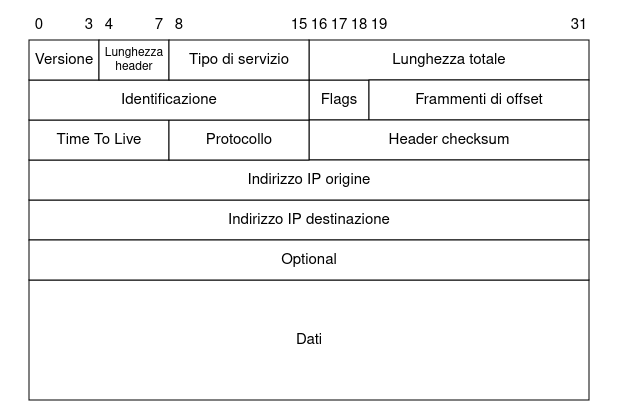
\includegraphics[width=0.75\linewidth]{Images/header_IP.png}
	\caption{Panoramica intestazione IP}
\end{figure}

\begin{comment}
	--- Livello di rete
	Il comportamento adesso riguarda ogni elemento della rete, quindi non solo più i due end-host, bensì anche i router.
	Analizziamo il protocollo IP (Internet Protocol), l'unico disponibile per questo livello. Definiamo il suo header.
	- Versione del protocollo 4b: Possono coesistere più versioni di IP, attualmente è in uso IPv4, ma esiste anche IPv6
	- Lunghezza dell'header: Lungo 20b se non ci sono opzioni, altrimenti è lungo 20b.
	- Lunghezza totale: Lunghezza di header e payload; indica globalmente la grandezza del pacchetto.
	- Service Type: Codice identificativo di una classe di servizio (nei router ci sono più buffer di uscita, dalla priorità più alta alla più bassa.
	In base al campo service type i pacchetti sono messi in coda al buffer più appropriato.)
	- Identification, flag e fragment offset sono legati alla frammentazione (vista più tardi)
	- TTL (Time to leave): Contatore inizializzato dalla sorgente (Di norma 64 o 128) che identifica il numero massimo di router che il pacchetto può
	attraversare. Alla ricezione di un pacchetto, ogni router decrementa di 1 questo valore. Se il valore arriva a 0, il router scarta il pacchetto e
	invia un messaggio di errore alla sorgente. Utile negli scenari di rerouting in caso di problemi sui link; si ricalcola il percorso e se è troppo
	lungo entra in gioco il TTL. Previene inoltre cicli infiniti.
	- TYPE: Codice che identifica il protocollo usato nei dati trasportati nel payload.
	- Header checksum: Esattamente come i precedenti checksum discussi.
	
	--- Frammentazione IP
	C'è un legame con la maximum transmission unit, perché ogni host ne ha una. Generalmente, data una tecnologia di trasmissione di Lv.2 (Data-link)
	c'è una dimensione massima di trasmissione che tale scheda di rete può gestire (Maximum Transmission Unit).
	Que pasa se un pacchetto incontra una scheda di rete con minore MTU del pacchetto durante il percorso?
	Il router con link di uscita con MTU < della dimensione del pacchetto frammenta quest'ultimo in più pacchetti con MTU compatibile con il link di
	uscita.
	I campi dell'header IP coinvolti sono:
	- Identification: Numero progressivo dato dalla sorgente al pacchetto IP (ATTENZIONE: NON HA RELAZIONI CON IL SEQUENCENUMBER DEL TCP). Tutti i
	frammenti del pacchetto avranno lo stesso numero identificativo del pacchetto frammentato.
	- Dei tre flags, uno è chiamato "M (More fragments)". Se è impostato a 0, il pacchetto non è stato frammentato oppure è l'ultimo frammento. Se è
	impostato a 1, è uno dei frammenti.
	- Offset: Posizione del frammento rispetto al pacchetto originario (diviso per 8).
	
	--- Esempio
	Supponiamo un MTU da 5000B e il pacchetto generato è da 4000B + 20B di header IP. Nel campo identification avrà avuto 476, il flag M è a 0, in
	quanto il pacchetto non è frammentato, e per la stessa ragione offset ha valore 0.
	Nel percorso, il pacchetto attraversa un router con link di uscita MTU 1420. 1400 per il payload, 20 per header IP. Il pacchetto sarà spezzato in
	tre e avremo:
	- srcIP, dstIP e identification uguali per ogni frammento.
	- Il valore del flag M sarà 0 nell'ultimo, negli altri sarà posto a 1.
	- L'offset per il primo è 0/8=0, il secondo è 1400/8=175, il terzo è 2800/8=350
	Con questa divisione i pacchetti potranno essere inviati e ricevuti in qualsiasi ordine; potranno essere ricostruiti grazie a M e offset.
	
	Ma chi effettua il riassemblaggio? Ovviamente l'host di destinazione. Non i router intermedi. L'end-host, proprio. Quando la destinazione riceve un
	frammento, fa partire un timer (generalmente di 250ms), se non riceve tutti i frammenti entro la sua scadenza, scarta tutto.
\end{comment}

%

\section{Protocolli di routing}
Distance vector, link state routing

\begin{comment}
--- Livello di rete - pt.2 (routing/instradamento)
Scopo del livello di rete è data una destinazione, fare il possibile per consegnare i pacchetti a tale destinazione. Il livello IP non dà nessuna
garanzia di consegna, per questo fa il possibile. Si dice infatti che IP sia un protocollo best effort; possono sussistere condizioni non ideali per la
perdita di pacchetti e IP non ha modo di recuperarli.
	Per UDP no problem, ma se TCP usa IP ha dei meccanismi per recuperarli. Il recupero non si trova quindi nel dominio operativo del livello di rete.
	Ci pensa quello di trasporto.
	
Parliamo ora di consegna diretta e indiretta. La consegna diretta è quando una destinazione appartiene alla stessa rete. (in IM1, da hostA a hostB).
Se la destinazione è in un'altra rete, è necessario demandare qualcuno (il router) per la consegna.
	Come fa un host a capire che tipo di consegna è?
	
Un host conosce oltre al proprio indirizzo IP, la maschera della rete a cui appartiene e l'indirizzo IP del router di bordo della rete a cui appartiene.

Data una destinazione (IP_d) l'host confronta (IP_h && mask) con un and bit a bit, facendo rimanere immutato il prefisso e mettendo il suffisso a 0.
Confronta questo valore con (IP_d && mask). Se i due valori sono uguali, allora la destinazione appartiene alla stessa rete e sarà una consegna diretta.
Altrimenti, se i due valori sono diversi, la destinazione apparterrà a un'altra rete e sarà consegna indiretta, richiedente l'appello del router di
bordo.

Il routing è il processo di scoperta del cammino migliore da una sorgente a una delle possibili destinazioni.
I router al loro interno mantengono una tabella di routing, dove per ogni destinazione è segnata l'interfaccia di uscita per arrivarci e un parametro
per il costo di attraversamento (di singolo hop, deduco).
	Il cammino migliore è determinato dai criteri adottati dall'ISP. Potrebbe fare più hop e costare più tempo ma meno in risorse, mentre potrebbe
	scegliere un cammino con meno hop per rapidità ma costare un pò di più.
	
Indovina indovinello, il routing passa attraverso un'astrazione con i grafi e diventa un problema di ricerca del cammino di costo minimo. I router sono
i nodi e i link sono gli archi, naturalmente. Per maggiori dettagli, vedasi la dispensa di algoritmi.
Il cacolo del cammino minimo avviene prima dell'attraversamento, ovviamente.

Lez12 - 28-04-26 Reti di calcolatori

--- Routing pt2
Data una topologia (quindi i router e i collegamenti), derivo il grafo e assegno i pesi in base a un determinato criterio. Normalmente il peso è
assegnato dall'amministratore di rete. Alcuni criteri sono:
	- Numero di hop attraversati: Soddisfatto ponendo tutti gli archi a peso 1. Il cammino minimo avrà valore minore di tutti.
	- Velocità di trasmissione (nominale del link): Pesi inversamente proporzionali alla banda, perché maggiore è la velocità, minore è il tempo usato 
	per il trasferimento.
	
Algoritmi per il calcolo del cammino minimo di un grafo possono essere:
	- (che considerano lo) Stato dei collegamenti (Link state routing algorithm): Algoritmo "centralizzato": Ogni router conosce la topologia della
	rete e calcola in autonomia il cammino minimo, decidendo poi il link di uscita.
	- Vettori distanza (Distance vector routing algorithm): Algoritmo distribuito; i router si parlano tra di loro ma non conoscono l'intera topologia
	della rete. Conoscono solo router adiacenti.
	- SDN (Software Defined Network): Algoritmo realmente centralizzato; c'è un'entità esterna che conosce la topologia intera che comunica col router
	e gli comunica le tabelle di routing per il cammino minimo.
	
Esistono uno o più protocolli per ciascuna categoria per l'implementazione degli algoritmi di routing. (guarderemo solo gli algoritmi, citeremo solo i
nomi degli algoritmi e ignoreremo il formato dei messaggi)
	Per far funzionare gl algoritmi i router si scambiano messaggi tramite specifici protocolli. Ciascun router invia periodicamente (il tempo dipende
	dal protocollo) ai propri router adiacenti un messaggio di aggiornamento. Il messaggio di routing contiene informazioni relative allo stato dei
	collegamenti (se le interfacce sono raggiungibili) ed è incapsulato con un header IP. srcIP è quello della sua interfaccia di uscita, dstIP è
	quello del router destinatario.
	
--- Algoritmi Link State
Ogni nodo della rete conosce l'intera topologia della rete e ogni nodo calcola autonomamente i cammini minimi da sé al nodo destinazione. Imposta le
proprie tabelle di routing di conseguenza.
	Sembrerebbe un algoritmo avido, che sceglie l'arco dal peso minore ogni volta. Si salva la strada da percorrere e scrive nella tabella di routing
	le interfacce migliori per ogni hop. Impostate tutte, i pacchetti sanno di dover utilizzare le interfacce di uscita segnalate. L'algoritmo
	utilizzato per raggiungere questo scopo è quello di Dijkstra.
	
In breve, i nodi si scambiano messaggi periodicamente per verificare se sono ancora raggiungibili mediante informazioni sui propri link. In caso di
guasti o cambio di topologia, la relativa informazione è immediatamente propagata per aggiornare la topologia e le proprie tabelle di routing.
Protocollo standard (che tutti i router devono supportare) basato su link state è OSPF (Open Shortest Path First).

--- Algoritmo distance vector
Supponiamo 3 nodi, i,j,k. i e j hanno un collegamento diretto (sono adiacenti, quindi), mentre l'altro no, sebbene rimanga raggiungibile.
Il costo dell'arco da i a j è c(i,j). Il costo di un cammino da i a k è D(i, k) = \sum c(l, n), dove l->n\in Cammino.
Quindi il costo è la somma dei costi dei singoli link che compongono il cammino. c è costo. D è distanza.

Supponiamo ora un nodo i e tre suoi adiacenti, j,l,m. Sono gli unici vicini diretti di i.
Ipotizziamo ora una destinazione k, per la quale j,l,m hanno calcolato la distanza con questa destinazione, quindi D(j,k), D(l,k), D(m,k).
Come troviamo D(i,k)? Il suo cammino minimo sicuramente deve passare per nodi adiacenti, quindi le uniche possibilità che abbiamo per ottenere D(i,k)
sono attraversare uno degli archi ai suoi nodi adiacenti e poi fare la somma con tutto il resto del cammino. Per esempio, se scelgo
j: D(i,k) = c(i,j) + D(j,k).
	Il cammino minimo sarà il costo minimo tra i cammini disponibili, naturalmente. Ma con questa osservazione capiamo che il nodo i non ha bisogno
	di conoscere la topologia, bensì solamente il costo minimo dell'hop.
	
In generale definiamo il costo del cammino minimo: D(i,k) = min(c(i,v) + D(v,k)), con v nodo adiacente a i.
Il calcolo della distanza minima è ripetuto ad ogni hop per scegliere l'arco di costo minore fino ad arrivare alla destinazione.
L'algoritmo usato è quello di Bellman-ford. Proviamo ad applicarlo ad un caso di esempio.

-- Esempio
Focalizziamoci sulla tabella di routing di A. La si inizializza, ottenendo i nodi adiacenti, i nextHop e il relativo costo.
Per esempio A->A non ha nextHop ed è a costo zero, A->B ha nextHop B e costo 7, etc.
Si inizializzano anche le tabelle dei nodi adiacenti E e B.
	Data questa inizializzazione, il nodo A nella prima iterazione riceve i distance vector del nodo B (A7, B0, C1, E5) e del nodo E (A1, B5, D2, E0).
Per la destinazione B, il nodo A calcola D(A, B) = \begin{cases}
	c(A, B)=7 + D(B, B)=0 \implies = 7\\
	c(A, E)=1 + D(E, B)=5 \implies = 6
\end{cases}
\noindent Siccome nella tabella c'era un costo iniziale da A verso B pari a 7, avendo trovato un costo minore attraverso E, il nodo A aggiorna la
tabella per la destinazione B con costo 6 e nextHop il nodo E. L'aggiornamento avviene per ogni destinazione contenuta nei DV ricevuti.

\end{comment}

%

\section{Protocollo ICMP}

%

\section{Protocollo di configurazione DHCP}

%

\section{IPv6}

%

\section{Network Address Translation - NAT}